\documentclass[../root]{subfiles}
\graphicspath{{_images/}{../_images/}}


\begin{document}

    \chapter{PROTECTIVE OR COUNTER-PRODUCTIVE?}

    \begin{shortsummary}
        \begin{itemize}
            \item \authoryear{Angrist2003}
            \item \RQ{How does immigration effect interacted with labour protect institution?}
            \item \answer{Empirical analysis using the cross-country panel data estimate immigration effect from Yugoslavia. And, it also estimate interacted with the country institution.}
            \item \result{Labor protection increases negative immigrant effect}
        \end{itemize}
    \end{shortsummary}

    \section{introduction}
    
    Many observers note that the increased immigration is likely to be part of any strategy to keep European social security system solvent. 
    However, the rise in immigration has been associated with high level  of anti-foreign sentiment and the view that immigration take jobs from natives is widespread(Bauer . et al.,2000). \\
    Rodrik(1997) has argued that the demand for social insurance is in part a response to to pressures of global economic integration, including migration.However, the equilibrium consequences of protective regulations and institution. \\
     This paper look at the employment consequence of immigration in Western Europe, motivated by two consideration.  
     \begin{enumerate}
         \item This paper use the Balkan War(1912-1913) as a immigration experiment along the lines of Card's(1990). 
         \item This paper focus on institutional aspects of the immigration question.
    \end{enumerate}
    {\bf Theoretical analysis}
    \begin{itemize}
        \item Institution may amplify any negative employment consequence at immigration for natives
    \end{itemize}
     
     {\bf Empirical analysis}
     \begin{itemize}
         \item This paper Use panel data set for European Economic Area (EEA) country for 1983-99.
         \item The Europe Commision's statistical agency (Eurostat) produced consistent time series of immigration measures and labour market variable by age, sex, education, and nationality or natives.
     \end{itemize}
     
     {\bf The advantage of these data set} \\
     This data set allow conduct analysis much like individual European countries using micro data, while allowing consistent cross-country comparisons.  \\
     
     {\bf IV strategy} \\
     Bias form endogenous mobility nay be mitigate by use of the two 1990's Balkan Wars(in Bosnia and Kosovo) as a source of exogenous variation providing shock to immigrant flow in Europe. \\
     
     Empirical analysis show immigration with interacted with institution affect negative effect.
     %ここから再度記述
    
    
    \section{Theoretical Framework}
    This paper analyse how immigration affect native employment using theoretical analysis.  It also show how the effect of immigration on native employment might be modified by institution such as firing costs.
    
    Firm output is assumed to be produced by immigrants and natives with production function:
    \begin{align*}
        f[\theta g(N_t, I_t)]; \\
        g(N_t, I_t)=(N_t+I_t)^{\frac{1}{\rho}},
    \end{align*}

    where $N_t$ and $I_t$ are the umber of natives and immigrants. The function $g(N_t, I_t)$ is CES labour aggregate function and $\theta$ is a location-specific shifter.

    An important feature of many European labour countries is high firing cost.
    Immigrants are likely to work in non-union jobs, on fixed-term contracts, or illegally.

    $\varphi$ is discount factor and Firm's present value of profit is as follow:

    \begin{align*}
        \Pi = \sum^{\infty}_{t=0} \varphi^t \{ f[\theta g(N_t, I_t)] -w_{N_t}N_t - w_{I_t}I_t - \lambda C_N N_{t-1} \},
    \end{align*}

    where $\lambda$ is a proportion of the labour force laid off each periods.
    We can simplify above equation as
    \begin{align}
        \Pi = (1-\varphi)^{-1} [f(\theta g)-w_N N -w_I I-\varphi \lambda C_N N]
    \end{align}
    Employment levels are chosen to satisfy F.O.C
    \begin{subequations}
        \begin{align}
            &f'(\theta g)\theta g_N =w_N + \varphi \lambda C_N=w_N(1+\varphi \lambda c_N) \\
            &f'(\theta g)\theta g_I=w_I,
        \end{align}
    \end{subequations}
    where $g_N$ and $g_i$ are derivatives of $g(N,I)$.$c_N$ is defined as a proportional to the native wage. \\
    The immigrant population is denoted by M, employed in $m$ identical firms, so that I=M/m.
    The native labour supply function is 
    \begin{align}
        N^*=[w_N (1-r)^{\epsilon}P],
    \end{align}
    where P is native population and r is the umemployment insurance replacement replacement rate, and $\epsilon$ is the native supply elasticity. \\
    In the short run(m is fixed), 
    \begin{align}
        \mbox{ln} \ f'[\theta g(N,I)] +\mbox{ln}\ \theta +\mbox{ln}\ g_N(N,I)= \mbox{ln} \ w_N +\mbox{ln} \ (1+\varphi \lambda C_N) \nonumber \\
        \approx \frac{1}{\epsilon} \mbox{ln}\frac{N}{P}+\frac{1}{\epsilon} \mbox{ln}m + \varphi \lambda C_N + r 
    \end{align}
    Eq(4) provide a basisfor this paper's emprical work.
    The short-run impact of immigration total native employment, $N^*\equiv mN$ and  the question of wheter $\frac{\partial N^*}{\partial M}$ changes with firing costs, $c_{N^{\cdot}}$, replacement rate, r, and the degree of native wage flexibility.
    The short-run employment impact of immigration can be written in elasticity terms as follow,
    \begin{align}
        \frac{d\mbox{ln} \ N^*}{d \mbox{ln} \ M}= \frac{\partial N}{\partial I}\frac{I}{N}= \xi _{NI}(\epsilon^{-1}-\xi _{NN})^{-1} \equiv e(N,\epsilon)
    \end{align}
    $\xi_{NN}=\frac{\partial w_N}{\partial N}\frac{N}{w_N}$ and $\xi_{NI}=\frac{\partial w_I}{\partial I}\frac{I}{w_I}$.
    If immigrants and natives are perfect substitution ($\rho=1$), then $\xi_{NI}$ and e(N,$\epsilon$) are necessary negative.
    The impact of changing in firing costs to the employment effect is as follow:
    \begin{align*}
        \frac{\partial e}{\partial N}\frac{\partial N}{\partial c_N} 
    \end{align*}
    
    {\bf The impact of firing cost} \\
    From the Eq(4), this paper show firing costs reduce employment in this model.
    \begin{align*}
        \frac{\partial N}{\partial c_n} = -\frac{\varphi \lambda}{\Delta}<0,
    \end{align*}
    where $\Delta$ is $\frac{1}{N}$ times te denominator in (5).

    The scale effect, $\frac{\partial e}{N}$, is likely to be positive and this is as follow.
    \begin{align*}
        \frac{\partial e}{\partial N}=\frac{\partial \xi_{NI}}{\partial N}(\epsilon^{-1}-\xi_{NN})^{-1}+ \xi_{NI}(\epsilon^{-1}-\xi_{NN})^{-2}\frac{\partial \xi_{NN}}{\partial N}
    \end{align*}
    Because the wage decline for natives from a given percentage are increase in immigrants is likely to be smaller, the first term is typically positive. The second term is negative if $\frac{\partial \xi_{NN}}{\partial N}$. Standard model of two factor constant-return model satisfy this condition.So, The impact of firing cost is negative.
    
    {\bf The impact of changing r} \\
    As same way, this paper check the impact of changing r as.
    \begin{align*}
        \frac{\partial e}{\partial r}=\frac{\partial e}{\partial N}\frac{\partial N}{\partial r}
    \end{align*}
    Higher replacement rates reduce native employment levels.
    \begin{align*}
        \frac{\partial N}{\partial r}=-\frac{(1-r)^{-1}}{\Delta}<0 
    \end{align*}
    
    {\bf The effect of Wage rigidity } \\
    Suppose that native wage is binding minimum or contract wage $\overline{w}_N$ and consider the effect of immigration.
    \begin{align*}
        \frac{\partial N^*}{\partial M}\frac{M}{N}= -\xi_{NI}\xi_{NN},
    \end{align*}]
    
    which is $e(N,\epsilon)$ with $\epsilon=\infty$, and is more negative than $e(N, \epsilon)$ with $\epsilon$ is unrestricted. \\
    
    {\bf Long-run effect} \\
    Assuming profits were equal to entry cost before immigration and the increase in profits  after immigration induce the entry of new firm.
    Because the entering firms employ additional workers, the possibility of endogenous entry reduce and may even eliminate any negative immigration impact.
    
    The effect of immigration on aggregate employment is
    \begin{align}
        \frac{\partial N^*}{\partial M} \frac{M}{N^*}=e(N,\epsilon)(1-\frac{\partial \mbox{ln} \ m}{\partial \mbox{ln} \ M})-\xi_{NN}(\epsilon^{-1}-\xi_{NN})^{-1}\frac{\partial \mbox{ln} \ m}{\partial \mbox{ln} \ M}
    \end{align}
    Since $\xi_{NN}$<0 and $\frac{\partial \mbox{ln} \ m}{\partial \mbox{ln} \ M}$<1, the response with entry is less than in the short-run case and can even be positive.

    \section{Background and Data}
    %dataの記述
    \begin{figure}[h]
        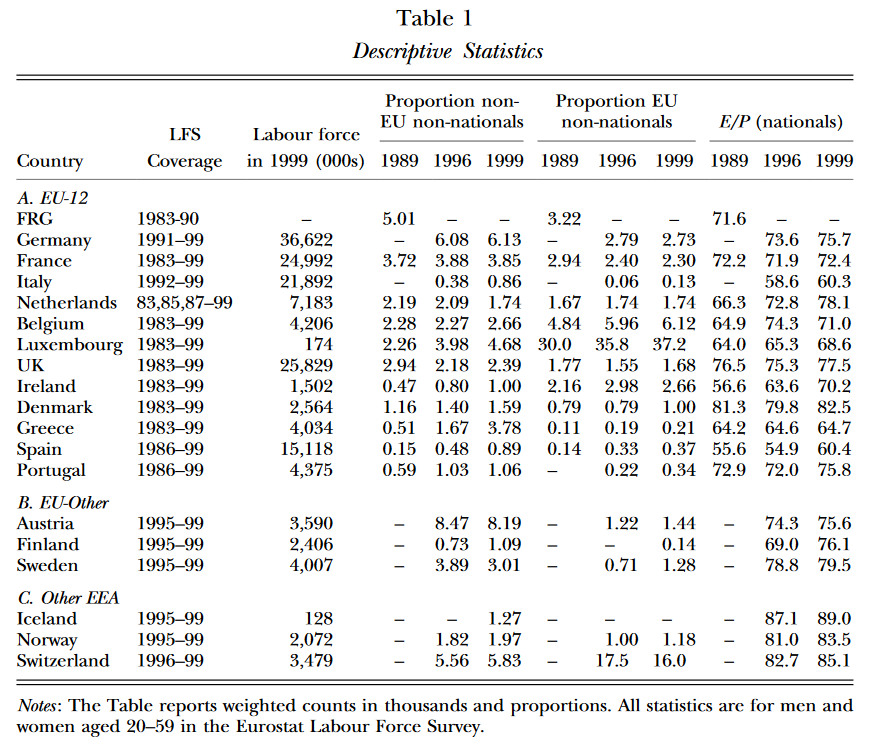
\includegraphics[width=15cm]{0529sugiyama/Table1.png}
    \end{figure}
    %出力にミス有 要確認
    The European countries with the largest proportion of labour force from non-EU countries have been Austria, France, Sweden, Switzerland and the UK.
    \begin{itemize}
        \item France and the UK absorb many immigration from former colonies.
        \item Germany and Austria accept large numbers of migrants from Turkey and Eastern Europe.
        \item Sweden accepts large immigrants from Middle Eastern countries. 
    \end{itemize}
     
    Migration within the EU is also important factor. In some countries accept the immigration from other developed European nations. 
    This paper distinguish between EU and no-EU foreigners, and use this distinguish to control for intra-EU migration that potentially responds to the number of non-EU immigrants. 

    \begin{figure}[h]
        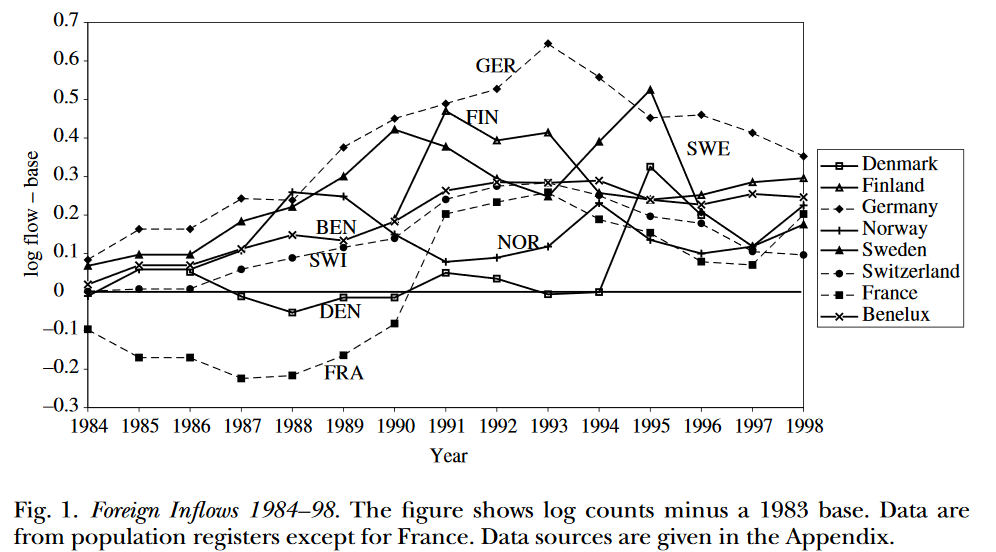
\includegraphics[width=15cm]{0529sugiyama/Figure1.png}
    \end{figure}
    There was less change in immigration up to 1988, but the early 1990s saw a marked upturn, especially Germany, France, and Sweden.
    \begin{figure}[h]
        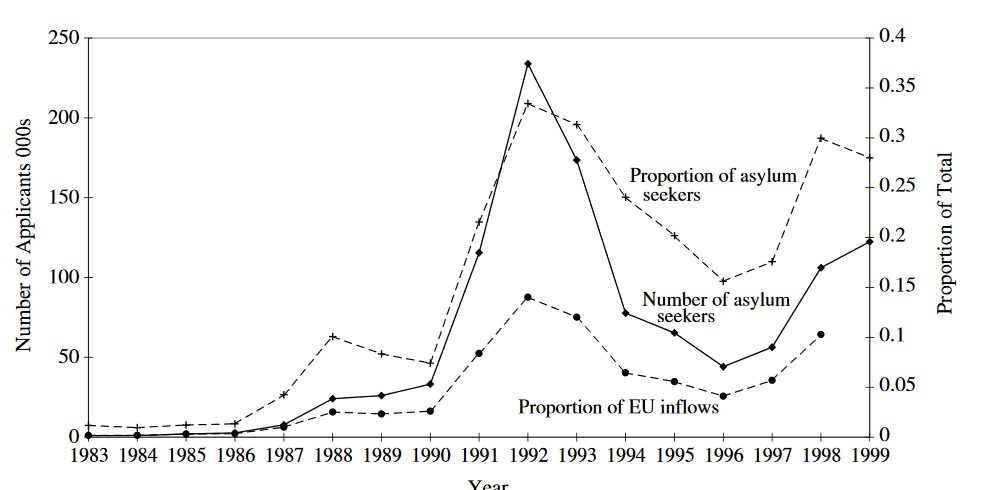
\includegraphics[width=15cm]{0529sugiyama/Figure2.png}
    \end{figure}
    The flow from Yugoslavia is large share of immigration in European countries after 1990.
    From table 2, the number of former Yugoslavia asylum-seeker peeked 1992, the year that Bosnia-Herzegovina independent state. \\
    Second peek is in 1999, when NATO launched air strikes in the Kosovo War.

    Many countries implement immigration policy. However, EU countries allow  Yugoslavia people to work, at least around the time of the Bosnia war. This paper use the data of the asylum-seeker from the Yugoslavia as treatment.

    \begin{figure}[h]
        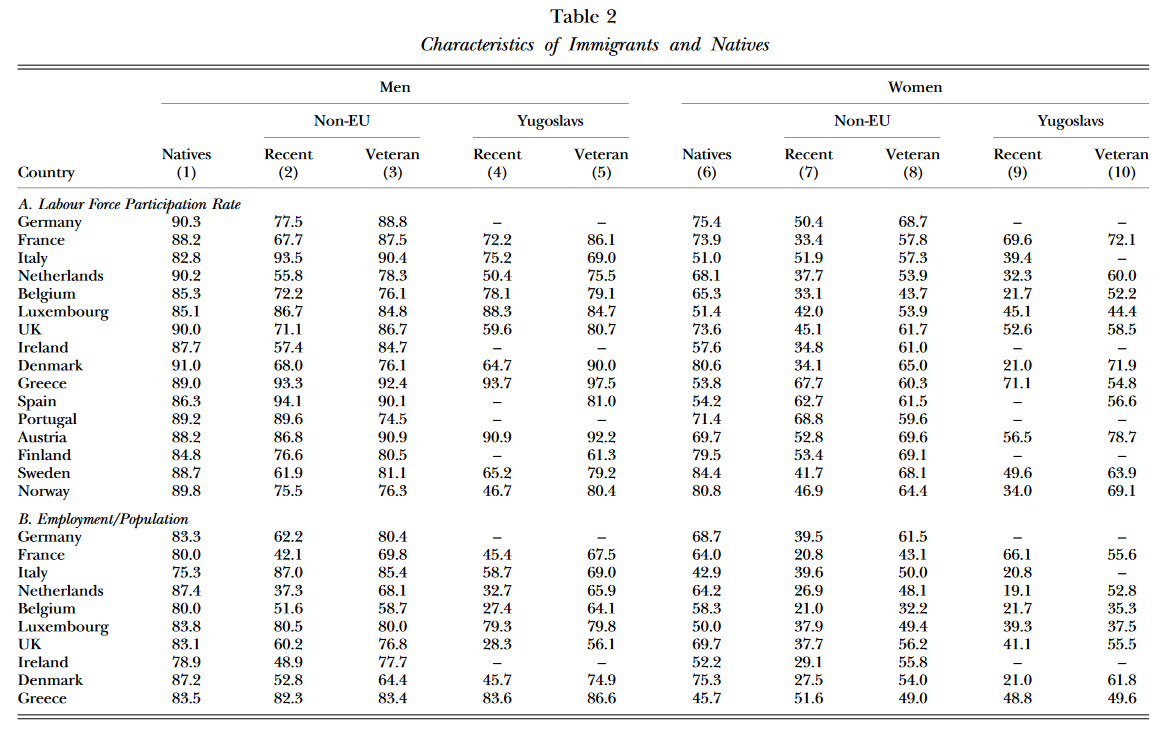
\includegraphics[width=15cm]{0529sugiyama/Table2.png}
    \end{figure}
    \begin{figure}[h]
        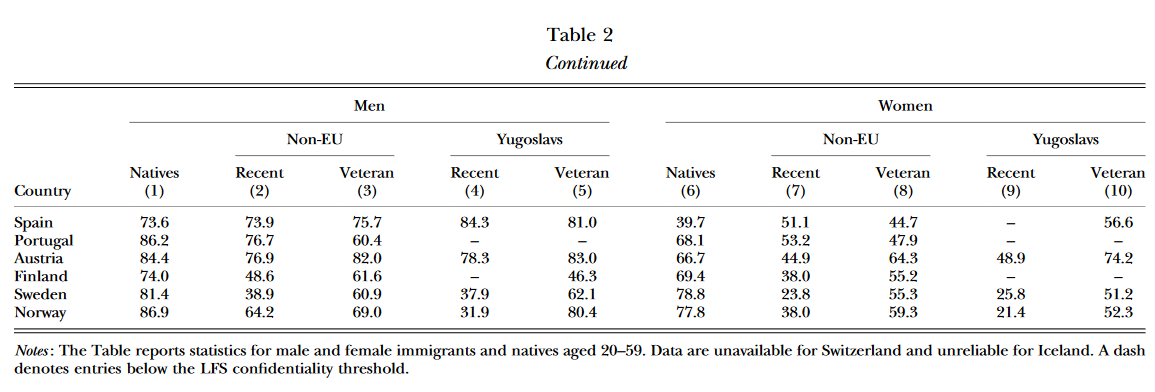
\includegraphics[width=15cm]{0529sugiyama/Table2(cont).png}
    \end{figure}

    In Table 2, this paper separate the immigrants into those arriving in the past 5 years(recent arrivals) and those arriving earlier(veteran immigrants). \\
    Participate rate for veteran male Immigrants are generally close to those for natives. \\
    Unemployment is typically higher among immigrants than native. From these results, we can check the gap between Participation rate and employment for immigrants is higher than for natives.
    
    
    \section{Estimates of Immigration Effect}
    The first equation estimated is 
    \begin{align}
        \mbox{ln} \ y_{ijt}= \mu_i + \delta_t + \beta_j +\alpha_i \mbox{ln} \ s_{jt} +\epsilon_{ijt}
    \end{align}
    for demographic group i, country j, and year t. The model includes country and year effect, $\beta_j$ and $\delta_t$.
    The regressor $\mbox{ln} \ s_{jt}$ is the log of the immigrant share and $y_{ijt}$ is the log of the employment-to-population ratio for natives. \\
    Equation(7) can be interpreted as approximating the F.O.C determining native employment.In this model, The variable of time-varying or labour demand shocks correlated both immigrants share and native employment is omitted. 
    So, This paper experimented with models that include controls for log of the foreign share with EU nationality, denoted $\mbox{ln} \ u_{jt}$.

    \begin{figure}[h]
        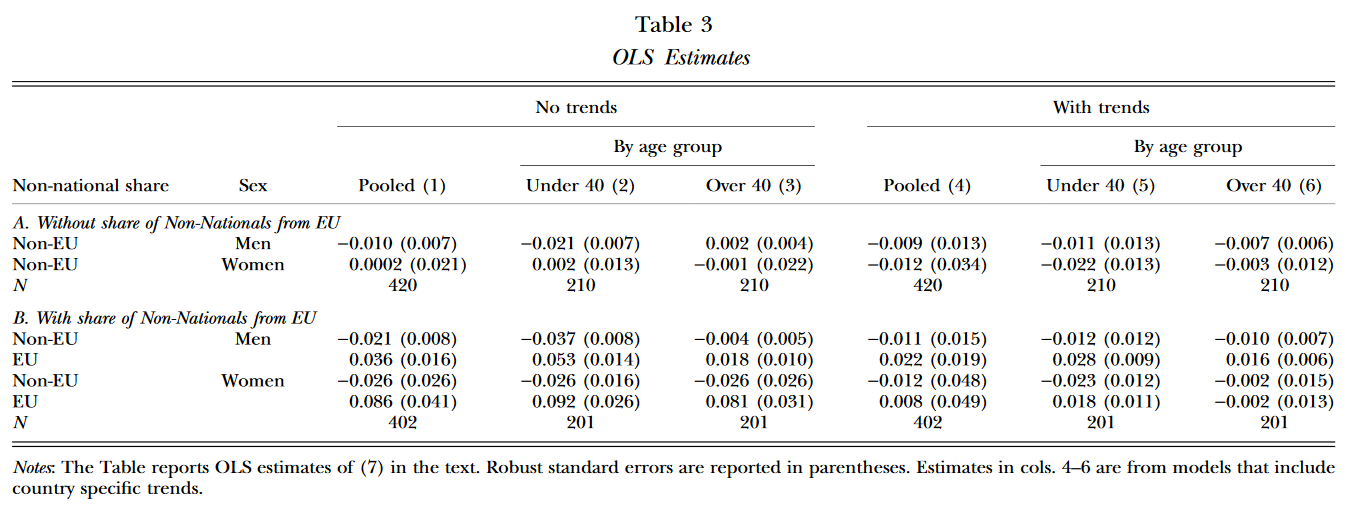
\includegraphics[width=15cm]{0529sugiyama/Table3.png}
    \end{figure}
    
    {\bf OLS estimates}
    \begin{itemize}
        \item The estimate of native men that omit the EU share show no significant effect at non-EU immigrants. 
        \item  The lager estimates generated by models that include the EU share are due to the fact that include the EU and non-EU foreign share are positive correlated.
        \item From the panel B, we can check the negative effect of non-EU immigration.
    \end{itemize}
    
    OLS estimates of the parameters in this equation are biased if immigration is correlated with country-specific trends.4-6 from models replacing the country effect,$\beta_j$, with a country-specific liner trend, $\beta_{0j}+\beta_{1j}t$. \\
    The estimate pooling age group are insignificant for both men and women. The inclusion of country trends does not necessary eliminate bias from endogenous immigration.

    {\bf IV strategy} \\
    The OLS may be biased upwards by immigrants choosing to locate where their employment prospect are best. So, this paper using IV strategy to estimate immigration impact.
    The choice of instruments is motivated by a sharp run-up in the number of Yugoslavs among European immigrants in the early and late 1990s. \\
    The first-stage equation for the IV estimates is 
    \begin{align}
        \mbox{ln} \ s_{jt} = \tau_{t} + \psi_{j} +b{jt} \pi_{b}+n_{jt}\pi_n+k_{jt} \pi_{k} +\eta_{ijt}
    \end{align}
    where 
    \begin{align*}
        b_{jt}&=\mbox{distance from the Sarajevo} \times \mbox{dummy for 1991-1995(Bosnia War year)} \\
        n_{jt}&=\mbox{distance from the Sarajevo} \times \mbox{dummy for 1996-1997(inter-war year)} \\
        k_{jt}&=\mbox{distance from the Pristina} \times \mbox{dummy for 1998-1999(Kosovo War year)}
    \end{align*}
    and $\tau_t$ and $\psi_t$ are year and country effects. \\
    As a specification check, this paper also estimate IV models with a parametric control for country-specific linear trends, as with the OLS estimate. 
    \begin{figure}[h]
        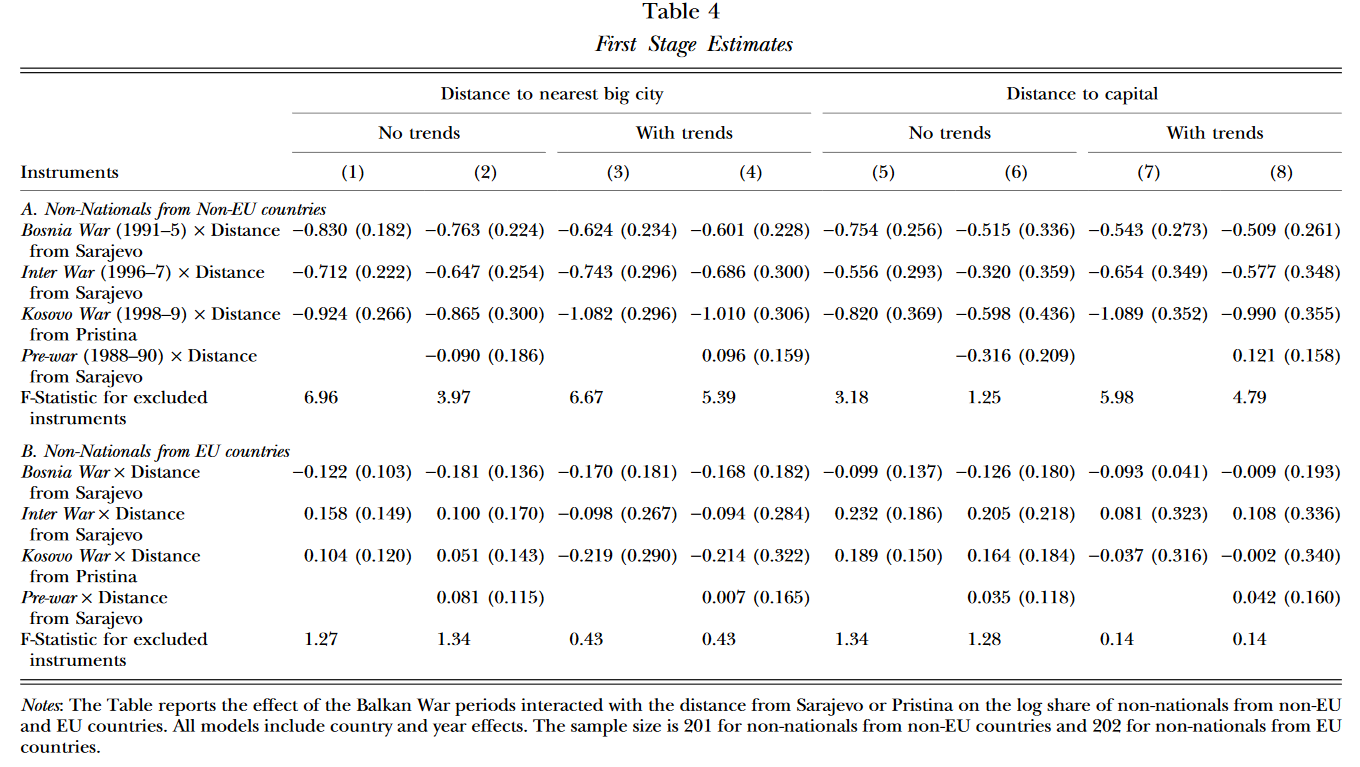
\includegraphics[width=15cm]{0529sugiyama/Table4.png}
    \end{figure}
    
    From panel A, 
    \begin{itemize}
        \item Immigration was highest during the war years.
        \item A moderate decline in the inter-war years.
        \item No evidence of a pre-exiting immigration trend
    \end{itemize}
    
    From panel B, 
    \begin{itemize}
        \item no relationship between war-rime interactions with distance to Sarajevo or Prinstina and EU share.
    \end{itemize}
    
    Because the first-stage relationship is stronger when distance is measured from large cities, this paper used this variable to construct the second-stage estimates. \\
    \begin{figure}[h]
        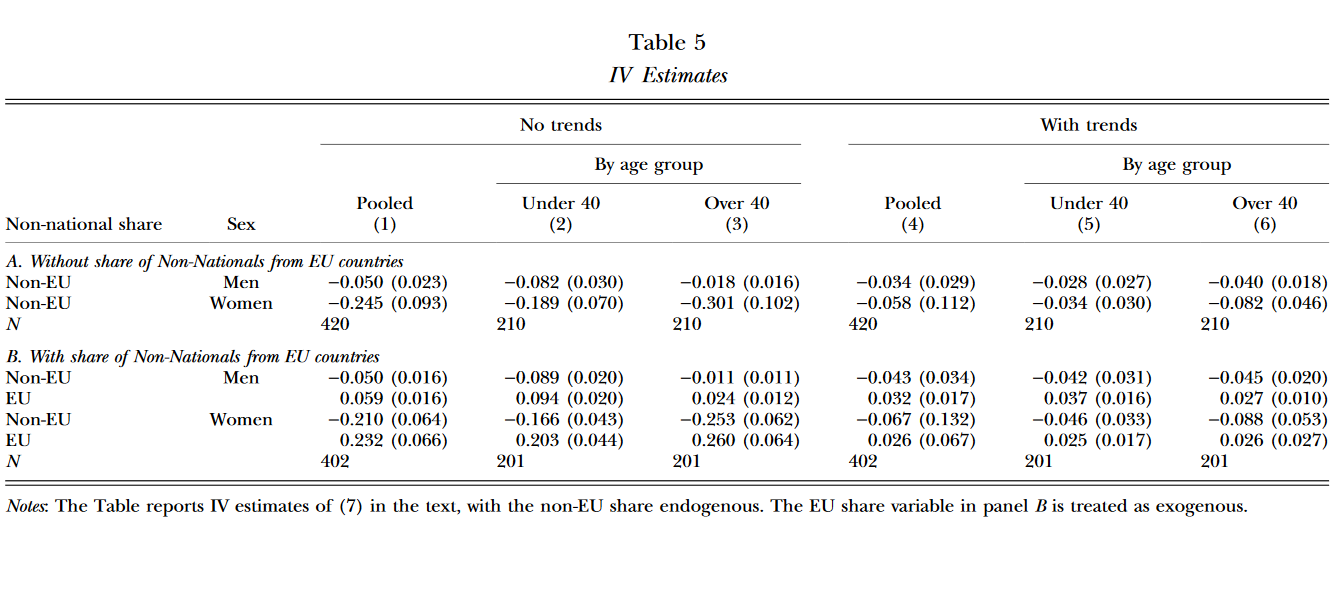
\includegraphics[width=15cm]{0529sugiyama/Table5.png}
    \end{figure}
    The 2SLS estimates using $b_{jt}, n_{jt} \mbox{and} k_{jt}$ as instruments are reported in Table 5. \\
    \begin{itemize}
        \item  For men, the effect is negative and significant both without and with trends.
        \item Women's negative effect may be too larger to be attributable to the effect of immigration.
    \end{itemize}
   
    One problem with the IV strategy for women is that some countries saw dramatic changes in female labour force participation (LFP) over this period while LFP in other countries was more stable.

    \section{Immigrants Interact with Institutions}
    Do institutions that labour and product market more rigid or less competitive change the employment consequence of immigrants for natives? 
    This paper looks at OLs and IV estimates of institutions with measure of three of the institutional features.
    
    \begin{itemize}
        \item employment protection
        \item replacement rate 
        \item labour market flexibility
    \end{itemize}
    The labour standard is that indexes the extent of employment protection, restrictions on work hours, and employment contracts. \\
    Replacement data is used average value. \\
    Interactions with a measure of entry costs taken from Nicoletti et al.(2000).
    
    Because the IV has problem for women, this paper analyses the effect of institution for only men.
    
    The equation used to estimate institution between immigrants and labour market institution Is
    \begin{align}
        \mbox{ln} \ y_{ijt} = \mu_i+\delta_t+\beta_j+(\alpha_{0i}+\alpha_{1i} \tilde{x_j})\mbox{ln} \ s_{jt} +v_{ijt}
    \end{align}
    where $\tilde{x_j}$ is an institutional characteristic, measured as the deviation from the median value in sample. \\
    $\alpha_{0i}$ is "Main Effect" and $\alpha_{1i}$ is "Interaction". This paper is interested in $\alpha_{1i}$.
   
    \begin{figure}[h]
        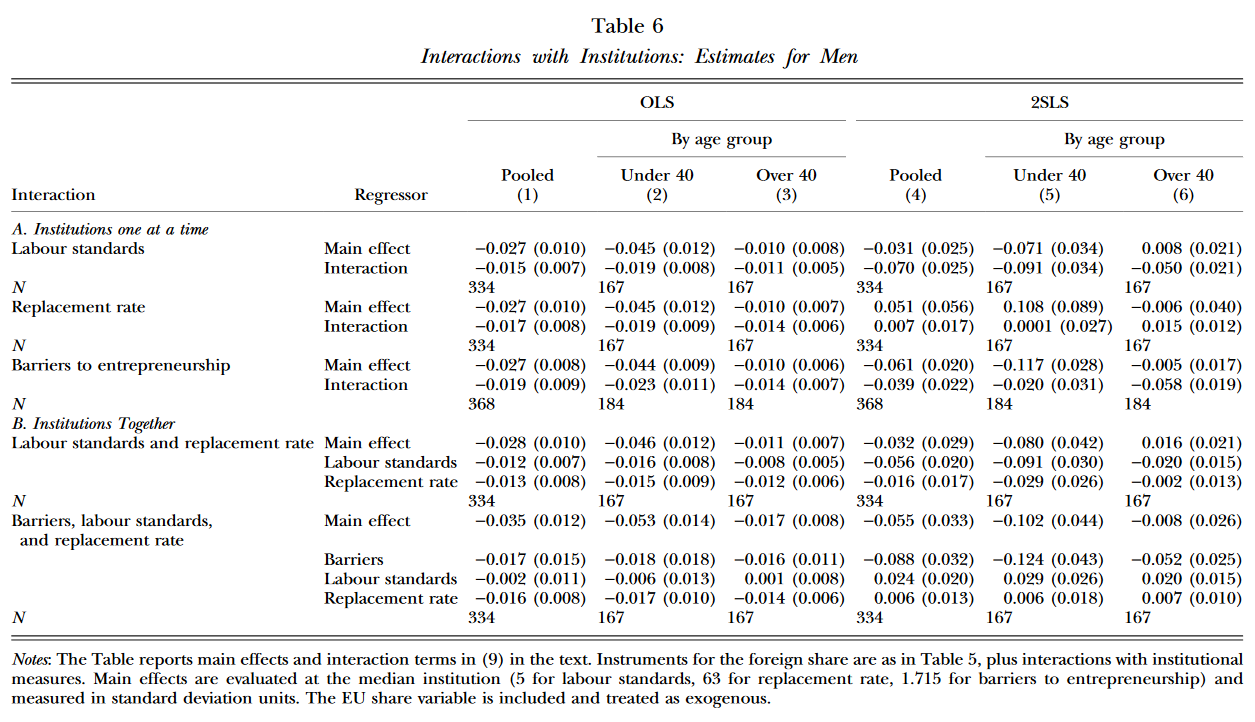
\includegraphics[width=15cm]{0529sugiyama/Table6.png}
    \end{figure}
    OLS Results are
    \begin{itemize}
        \item The interactive term are lager for young men than for over 40. 
        \item The effects of including both interactions are smaller than, and larger for younger men.
    \end{itemize}
    
    The 2SLS results are
    \begin{itemize}
        \item The labour standard negative effects are larger but less precise. 
        \item Entry barriers is only significant.
    \end{itemize}
    
    The stronger evidence of negative interactions with labour standards with replacement rate is consistent with theory, which attributes interactions with replacement rate solely to scale effect.
    
    \begin{figure}[h]
        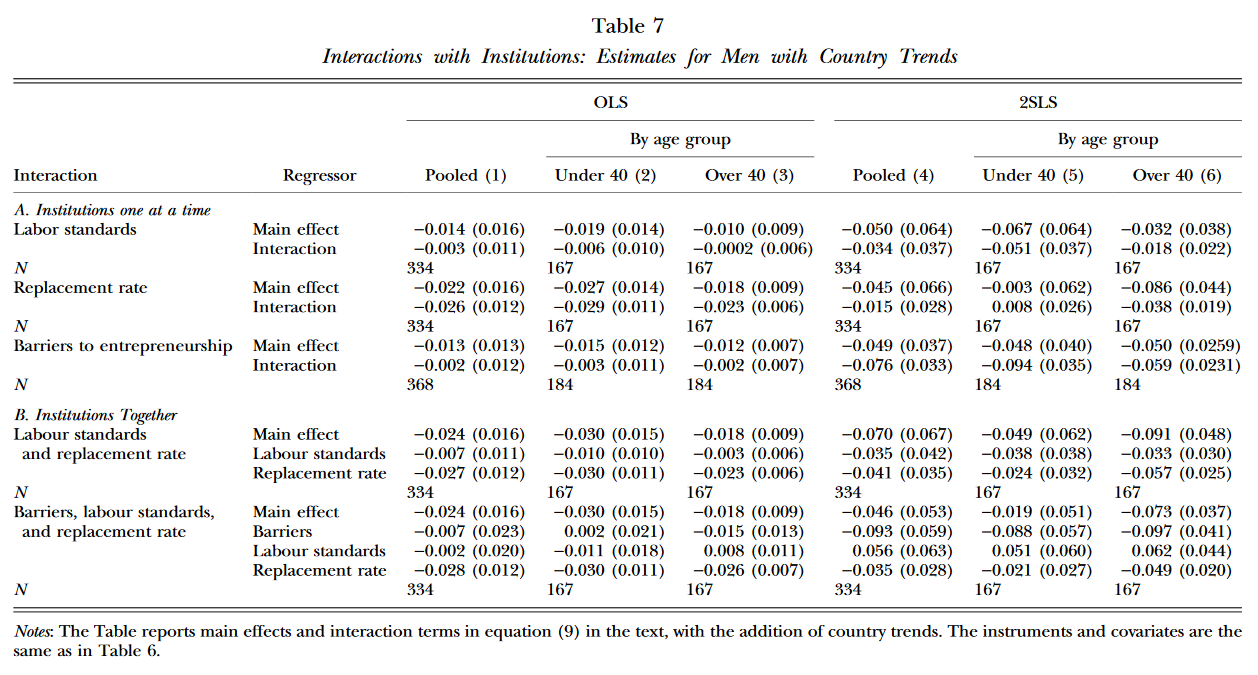
\includegraphics[width=15cm]{0529sugiyama/Table7.png}
    \end{figure}
    
    The results with countries trends show mostly negative and sometimes significant interactions, with no significant positive estimates.
    
    \section{summary and Conclusion}
    Though restrictive economic institutions can play a protective role for natives, may aggravate the negative impact of immigration on equilibrium native employment. \\
    Higher entry barriers and reduced wage flexibility  increase the negative impact of immigrants on native employment. \\
    Effect of this size may also signal interpret  and IV are not precise.It therefore  seems reasonable to interpret the OLS and IV estimates as bracketing the true effect.
    These negative interactions are apparent in the OLS and many of the IV estimates, though the IV estimates of interaction terms are less precise.\\
    Specific channels for interactions are difficult to identify.
    \biblio
    
    
\end{document}